\chapter{Experimental Results}
\label{chap:experimental-results}

This chapter reports the recorded monitoring window from 15~March to 6~July~2026 for the 12 recurring monitoring series and the later common-case deployment comparison for the eight candidate models with shared full-benchmark outputs on 22~May~2026.

\section{Monitoring results}
\label{sec:drift-results}

The timeline contains 187 eligible runs. The recurring monitored series are \texttt{claude-haiku-4-5}, \texttt{claude-sonnet-4-5}, \texttt{claude-sonnet-4-6}, \texttt{gemini-2.5-flash}, \texttt{gpt-4.1-mini}, \texttt{gpt-4.1-nano}, \texttt{gpt-5}, \texttt{gpt-5-mini}, \texttt{gpt-5-nano}, \texttt{gpt-5.1}, \texttt{gpt-5.2}, and \texttt{gpt-5.4}. For each recurring model, the first recorded run was a full-benchmark baseline on \(\mathcal{D}_N\); later routine monitoring runs used the frozen \(n=300\) panel, and paired monitoring comparisons restricted both runs to the common panel items. These twelve recurring model labels therefore contribute 185 runs and 173 baseline-to-later paired comparisons. Missing outputs are removed pairwise, so the effective sample size can be below 300.

The two singleton labels are \texttt{gemini-2.0-flash} and \texttt{gpt-5.4-2026-03-05}; each appears once. A model's first recorded run is its full-benchmark baseline, so these two runs remain recorded baselines until a later comparison exists. The frozen labelled sets make this straightforward:
\begin{enumerate}
    \item a newly released model is scored on the same posts as the existing candidates;
    \item its first run is compared with the other series from the same period;
    \item later runs are paired against that model's own first-run baseline.
\end{enumerate}

At the one-sided nominal level \(\alpha=.05\), three comparisons produced monitoring signals with \(p_{\mathrm{exact}}<.05\). These signals opened review on the fixed panel; deployment significance was determined separately.

\begin{table}[htbp]
    \centering
    \small
    \caption{Canonical monitoring summary, 15~March--6~July~2026.}
    \label{tab:canonical-monitoring-summary}
    % Generated from canonical_summary.json; do not edit.
\begin{tabular}{lr}
\toprule
Quantity & Value \\
\midrule
Eligible scheduled runs & 187 \\
Models with comparisons & 12 \\
Baseline-to-later comparisons & 173 \\
Nominal one-sided \(p<0.05\) & 3 \\
\bottomrule
\end{tabular}

\end{table}
\provline{P4}

\begin{figure}[htbp]
    \centering
    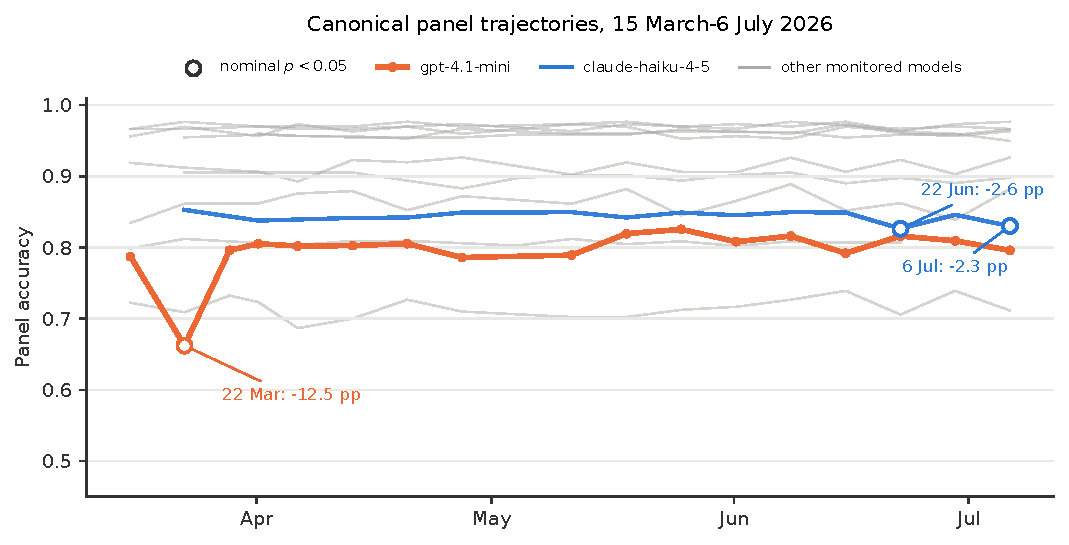
\includegraphics[width=\linewidth]{assets/evidence/fig_canonical_monitoring_trajectory.pdf}
    \caption[Canonical panel-accuracy trajectories]{Panel accuracy for the 12 recurring monitoring series. Open markers show the three nominal one-sided \(p_{\mathrm{exact}}<.05\) signals. The orange and blue trajectories identify the two models that produced them; grey series provide same-period context.}
    \label{fig:canonical-monitoring-trajectory}
\end{figure}
\FloatBarrier

Table~\ref{tab:nominal-mcnemar} reports the paired correctness counts for the three comparisons with nominal one-sided signals. McNemar's test uses the discordant cells: \(b\) counts items that changed from correct to wrong, and \(c\) counts items that changed from wrong to correct. The three comparisons are:
\begin{enumerate}
    \item \texttt{gpt-4.1-mini}, 15~March--22~March: \(b=49\), \(c=12\), \(n=296\);
    \item \texttt{claude-haiku-4-5}, 22~March--22~June: \(b=9\), \(c=2\), \(n=265\);
    \item \texttt{claude-haiku-4-5}, 22~March--6~July: \(b=7\), \(c=1\), \(n=265\).
\end{enumerate}

None of these two models were deployed in production, so no production deployment change was made.
\begin{table}[htbp]
    \centering
    \small
    \caption[Nominal McNemar tables]{Paired correctness counts for the three comparisons with one-sided \(p_{\mathrm{exact}}<.05\).}
    \label{tab:nominal-mcnemar}
    % Generated from baseline_to_later_mcnemar.csv; do not edit.
\begin{minipage}[t]{0.32\linewidth}
\centering
\texttt{gpt-4.1-mini}\\
{\scriptsize 15~Mar--22~Mar, \(n=296\)}\\[3pt]
\begin{tabular}{c|cc}
 & later \(+\) & later \(-\) \\
\hline
base \(+\) & 184 & \(b=49\) \\
base \(-\) & \(c=12\) & 51 \\
\end{tabular}\\[3pt]
{\scriptsize \(\Delta=-12.5\)\,pp, \(p_{\mathrm{exact}}=9.849\times10^{-7}\)}
\end{minipage}
\hfill
\begin{minipage}[t]{0.32\linewidth}
\centering
\texttt{claude-haiku-4-5}\\
{\scriptsize 22~Mar--22~Jun, \(n=265\)}\\[3pt]
\begin{tabular}{c|cc}
 & later \(+\) & later \(-\) \\
\hline
base \(+\) & 217 & \(b=9\) \\
base \(-\) & \(c=2\) & 37 \\
\end{tabular}\\[3pt]
{\scriptsize \(\Delta=-2.64\)\,pp, \(p_{\mathrm{exact}}=0.0327\)}
\end{minipage}
\hfill
\begin{minipage}[t]{0.32\linewidth}
\centering
\texttt{claude-haiku-4-5}\\
{\scriptsize 22~Mar--6~Jul, \(n=265\)}\\[3pt]
\begin{tabular}{c|cc}
 & later \(+\) & later \(-\) \\
\hline
base \(+\) & 219 & \(b=7\) \\
base \(-\) & \(c=1\) & 38 \\
\end{tabular}\\[3pt]
{\scriptsize \(\Delta=-2.26\)\,pp, \(p_{\mathrm{exact}}=0.0352\)}
\end{minipage}

\end{table}
\provline{P4}
\FloatBarrier

\paragraph{The March signal and rebound.}
For \texttt{gpt-4.1-mini}, the 15--22~March comparison in Table~\ref{tab:nominal-mcnemar} produced the strongest signal. Panel accuracy fell from \(0.7872\) to \(0.6622\), a change of \(-12.5\) percentage points, and the one-sided exact p-value was \(9.849\times10^{-7}\).

The next run, 22--28~March, reversed the movement: on 297 complete pairs accuracy rose from \(0.6633\) to \(0.7946\), with 11 regressions and 50 improvements. From 15 to 28~March the net change was \(+0.67\) percentage points, so the episode did not persist. \texttt{gpt-4.1-mini} was only a monitored candidate, therefore no production deployment change.

No model-specific incident or update notice for \texttt{gpt-4.1-mini} was listed in the public OpenAI status history for 15 or 22~March~2026~\cite{openai2026status}. The episode therefore illustrates the intended role of the monitor: it surfaced an unexplained provider-side behaviour change on the fixed panel without any contemporaneous public notice for that model was available.
\provref{P4}

\begin{figure}[htbp]
    \centering
    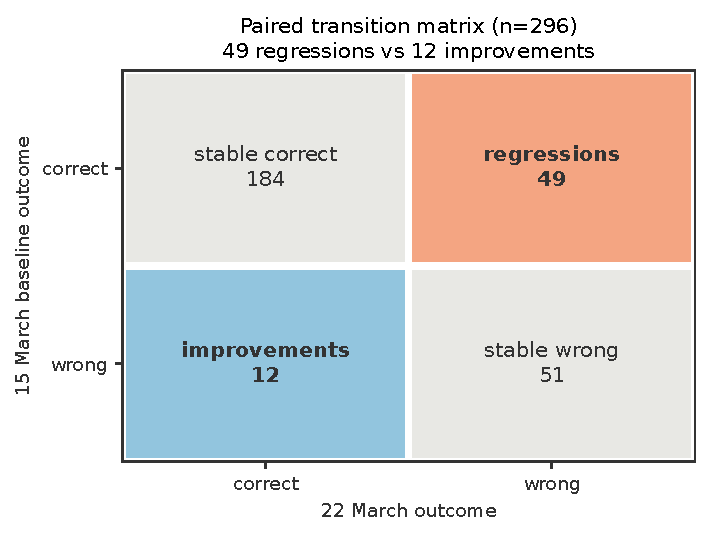
\includegraphics[width=0.68\linewidth]{assets/evidence/fig_canonical_mcnemar_matrix.pdf}
    \caption[Paired transitions behind the March signal]{Paired correctness transitions for \texttt{gpt-4.1-mini}, 15--22~March. McNemar's test ignores the two grey concordant cells and evaluates the imbalance between 49 regressions and 12 improvements.}
    \label{fig:canonical-mcnemar-matrix}
\end{figure}
\FloatBarrier

\section{Monitoring cost}
\label{sec:monitoring-cost}

\begin{table}[htbp]
    \centering
    \small
    \caption[Observed panel and benchmark API costs]{Observed API cost per evaluation sweep. The production set is \texttt{gpt-5-mini}, \texttt{gpt-5-nano}, and \texttt{gpt-5}.}
    \label{tab:monitoring-cost}
    % Generated from assets/drift/monitoring_cost.json; do not edit.
\begin{tabular}{lrr}
\toprule
Evaluation scope & Eight models & Three production models \\
\midrule
Full benchmark & \$43.10 & \$9.53 \\
Sentinel panel & \$12.26 & \$2.74 \\
\bottomrule
\end{tabular}

\end{table}

That paired sensitivity is inexpensive enough to run routinely. For the three production models---\texttt{gpt-5-mini}, \texttt{gpt-5-nano}, and \texttt{gpt-5}---one panel sweep cost \(\$2.74\), compared with \(\$9.53\) for a full-benchmark sweep. Weekly panel monitoring therefore costs approximately \(\$142.42\) per year in API charges.

The error cost of an undetected episode can be estimated conditionally on the penalties used in Section~\ref{sec:cost-aware-comparison}. On the 296 items shared by the \texttt{gpt-4.1-mini} baseline and signal runs, the confusion counts changed from \((\mathrm{FP},\mathrm{FN})=(2,61)\) to \((0,100)\). Holding inference price fixed, the resulting incremental error loss per affected classification is
\[
    \Delta L_{\mathrm{err}}
    =\frac{0.155(0-2)+0.031(100-61)}{296}
    =\$0.003037.
\]

\begin{table}[htbp]
    \centering
    \small
    \caption[Production-model monitoring scenarios]{Model-specific monitoring costs and break-even volumes under the observed episode's incremental error loss of \(\$0.003037\) per affected classification. Costs are USD; annual panel cost is \(52\times\) weekly panel cost, and weekly break-even volume is \(\text{panel cost}/0.003037=\text{annual panel cost}/(52\times0.003037)\).}
    \label{tab:production-monitoring-scenarios}
    % Generated from assets/drift/monitoring_cost.json; do not edit.
\begin{tabular}{lrrrr}
\toprule
Model & Panel & Full & Annual panel & Weekly break-even \\
\midrule
\texttt{gpt-5-mini} & \$0.43 & \$1.54 & \$22.37 & 142 posts \\
\texttt{gpt-5-nano} & \$0.11 & \$0.39 & \$5.79 & 37 posts \\
\texttt{gpt-5} & \$2.20 & \$7.60 & \$114.26 & 723 posts \\
\bottomrule
\end{tabular}

\end{table}
\provline{P5}

For the three production models, weekly panel cost ranges from \(\$0.11\) to \(\$2.20\), and the corresponding break-even volume ranges from 37 to 723 affected classifications under this scenario. Other failure patterns imply different thresholds. This supports the operational case for running the fixed panel routinely as a review trigger; model replacement still depends on the separate full-benchmark comparison in Section~\ref{sec:cost-aware-comparison}.

\section{Cost-aware comparison}
\label{sec:cost-aware-comparison}

The deployment comparison uses the 22~May common complete-case intersection for the eight candidate models with shared full-benchmark outputs on that date: 1113 items observed for all eight models. This avoids changing the evaluated item set across candidates. The illustrative operating point is
\[
    w=\frac{C_{\mathrm{FN}}}{C_{\mathrm{FP}}}=0.2,
    \qquad
    \lambda=C_{\mathrm{FP}}+C_{\mathrm{FN}}=0.186,
\]
which is equivalent to \(C_{\mathrm{FP}}=0.155\) and \(C_{\mathrm{FN}}=0.031\) USD, in addition to mean inference cost. At this operating point, a false positive is assigned five times the cost of a false negative. This reflects the operational burden of sending irrelevant posts into downstream processing.

\begin{table}[htbp]
    \centering
    \small
    \caption{Complete-case results on 22~May 2026 (\(n_t=1113\)); \(w=0.2\), \(\lambda=0.186\).}
    \label{tab:canonical-cost-comparison}
    % Generated from deployment_cost_may22.csv; do not edit.
\begin{tabular}{lrrrrrrr}
\toprule
Model & Accuracy & Precision & Recall & $c_t(m)$ (USD) & FP & FN & Loss \\
\midrule
\texttt{gpt-5-mini} & 0.940 & 0.991 & 0.901 & 0.0013 & 5 & 62 & 0.0037 \\
\texttt{gpt-5-nano} & 0.901 & 0.992 & 0.834 & 0.0003 & 5 & 105 & 0.0039 \\
\texttt{gpt-5.1} & 0.972 & 0.973 & 0.976 & 0.0053 & 16 & 15 & 0.0080 \\
\texttt{gpt-5} & 0.978 & 0.966 & 0.995 & 0.0065 & 21 & 3 & 0.0095 \\
\texttt{gpt-4.1-mini} & 0.754 & 0.994 & 0.572 & 0.0019 & 2 & 271 & 0.0097 \\
\texttt{gpt-5.2} & 0.979 & 0.973 & 0.989 & 0.0084 & 16 & 7 & 0.0108 \\
\texttt{gpt-4.1-nano} & 0.778 & 0.897 & 0.681 & 0.0007 & 49 & 198 & 0.0130 \\
\texttt{gpt-5.4} & 0.970 & 0.970 & 0.976 & 0.0115 & 18 & 15 & 0.0144 \\
\bottomrule
\end{tabular}

\end{table}
\provline{P5}

\texttt{gpt-5-mini} minimises plug-in loss at \(0.003698\). It balances low inference cost with five false positives and 62 false negatives. The cheaper \texttt{gpt-5-nano} is a close second at \(0.003950\): its lower inference cost does not offset 105 false negatives. The accuracy leader \texttt{gpt-5.2} reaches \(0.97932\) accuracy but has loss \(0.010835\), mainly because its inference cost and 16 false positives are expensive under the stated business asymmetry. Therefore neither maximum accuracy nor minimum API price alone selects the preferred deployment model.

\begin{figure}[htbp]
    \centering
    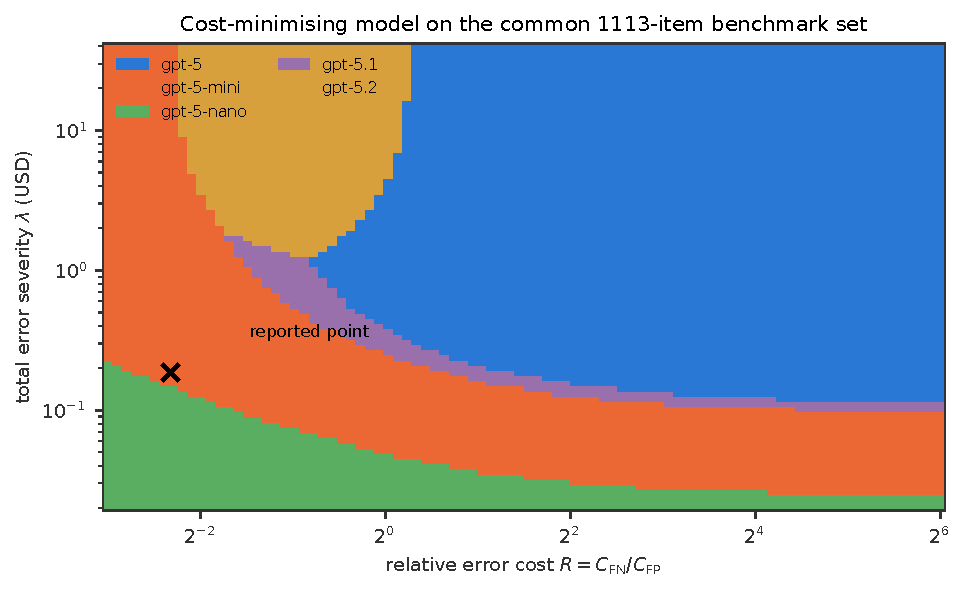
\includegraphics[width=0.9\linewidth]{assets/evidence/fig_canonical_cost_decision_map.pdf}
    \caption[Cost-minimising model over error-cost assumptions]{Model minimising the empirical plug-in loss over relative false-negative cost \(w\) and total error severity \(\lambda\). The cross marks the operating point reported in Table~\ref{tab:canonical-cost-comparison}. Large regions with different winners show why the result is conditional on declared penalties.}
    \label{fig:canonical-cost-decision-map}
\end{figure}
\provline{P5}

At the declared operating point, \texttt{gpt-5-mini} beats \texttt{gpt-5-nano} by only \(2.52\times10^{-4}\) USD per request. The margin is therefore small, and a modest change in the assumed penalties can change the winner. 
